\section{CGQ Model and Motivation}
\label{sec:background}

Following the style of recent database graph systems, this section first defines the computation model and then derives the design from measured workload properties.  The low-level GPU mapping is deferred to Section~\ref{sec:implementation}.

\subsection{Concurrent Graph Query Model}

Let $G=(V,E)$ be a directed graph stored once in device memory.  A query window contains $N$ source-based iterative queries over $G$.  At most $Q\leq64$ queries are resident in one batch; larger windows are divided into batches.  Query $q$ maintains a value $x_q(v)$ for every vertex and a frontier $\frontier_q^{\ell}$ at logical level $\ell$.  BFS stores distance and discovery state, SSSP stores weighted distance, and widest-path traversal stores a bottleneck value.  Correct CGQ execution must return the same value vector for every query as independent level-synchronous execution.

At global iteration $t$, query $q$ is either inactive or at logical level $\ell_q(t)$.  We define its exact union frontier and the query membership of each active vertex as
\begin{align}
  U_t &= \bigcup_{q\text{ active}} \frontier_q^{\ell_q(t)}, \\
  \querymask_t(v) &= \{q \mid v\in\frontier_q^{\ell_q(t)}\}.
\end{align}
$U_t$ identifies neighborhoods that may be reused; $\querymask_t(v)$ identifies exactly which queries may reuse the neighborhood of $v$.  A compact word represents the membership set for the current prototype, but the model itself is independent of that representation.

We target a closed query window over one static, GPU-resident graph.  Query sources may differ and queries may start at different global iterations.  Dynamic graphs, continuous arrival control, and multi-GPU partitioning are outside the central claim and are discussed in Section~\ref{sec:limitations}.

\subsection{Optimization Objective}

A CGQ system makes three coupled decisions for a query window $W$.  It partitions the queries into resident batches $\mathcal{B}$, assigns each query a bounded start offset $o_q$, and selects an access strategy $a_t$ at every global iteration.  We denote a complete choice by
\begin{equation}
  \Pi(W)=\langle\mathcal{B},\{o_q\}_{q\in W},\{a_t\}_{t\geq 0}\rangle.
\end{equation}
The batch and offsets determine which query frontiers coexist; the iteration strategy determines how the resulting graph and state work is accessed.  Optimizing any one choice in isolation can be misleading: a good strategy cannot share queries placed in different batches, while aggressive alignment can add more delay than the saved execution time.

Our primary objective is to minimize query-window completion time
\begin{equation}
  T(W,\Pi)=T_{\mathrm{schedule}}+T_{\mathrm{execute}}
  \label{eq:window-objective}
\end{equation}
subject to a resident-memory budget and per-query result equivalence with independent execution.  Query-dependent grouping, offsets, feature collection, and strategy selection are therefore online costs.  Reusable graph analysis is reported separately with its construction, storage, load, and break-even costs.  P50 and P95 query latency complement the window objective so that delaying a query to create sharing cannot appear free.

The system must select one policy without knowing the fastest alternative in advance.  Per-graph or per-query hindsight may characterize an upper bound, but it is not a deployable configuration.  The main evaluation consequently freezes the scheduling and strategy-selection policy and reports an oracle only as diagnostic evidence.

\subsection{A Memory-Access View of CGQ}

Independent frontier expansion accesses
\begin{equation}
  E_{\mathrm{ind}}(t)=
    \sum_q\sum_{v\in\frontier_q^{\ell_q(t)}}\deg^+(v)
\end{equation}
adjacency entries.  If every active vertex is processed once for the entire batch, the topology-access count becomes
\begin{equation}
  E_{\mathrm{union}}(t)=\sum_{v\in U_t}\deg^+(v).
\end{equation}
The normalized neighborhood-sharing opportunity is
\begin{equation}
  S_{\mathrm{share}}(t)=1-\frac{E_{\mathrm{union}}(t)}
                                    {E_{\mathrm{ind}}(t)}.
\end{equation}
It is zero for disjoint frontiers and approaches one when many queries simultaneously contain the same high-degree vertices.

Sharing the topology does not remove query-specific relaxations.  Their logical count is
\begin{equation}
  E_{\mathrm{pair}}(t)=
    \sum_{v\in U_t}\deg^+(v)\,\mathrm{popcount}(\querymask_t(v)).
\end{equation}
This distinction prevents an apparent reduction in adjacency access from hiding false query--edge work.  $E_{\mathrm{union}}$ captures how many graph entries need to be fetched, while $E_{\mathrm{pair}}$ bounds how much query-specific state must be examined.

Memory overhead is not determined by access count alone.  The remaining state accesses may be irregular and separately fetched, or may follow a regular order that lets the memory system serve several useful values together.  We therefore organize the design around two levers:
\begin{enumerate}
  \item \emph{access-count reduction}: reduce repeated neighborhood accesses from $E_{\mathrm{ind}}$ toward $E_{\mathrm{union}}$; and
  \item \emph{access-cost reduction}: organize the necessary $E_{\mathrm{pair}}$ state work to reduce the number and exposed latency of memory requests.
\end{enumerate}
This is a conceptual decomposition, not a claim that software changes the physical latency of DRAM.  The evaluation must connect neighborhood counts and state-access behavior to measured data movement, exposed stalls, and end-to-end time.

\subsection{Pilot Characterization}

We examined existing runs from the current prototype before finalizing the design.  These measurements are not production traces or final headline results; they establish the phenomena that a CGQ system must explain.  Table~\ref{tab:pilot-observations} summarizes the observations.

\begin{table*}[t]
  \centering
  \caption{Pilot observations from the current V100 prototype.  They motivate the memory-access design but are not extrapolated beyond the measured workloads.}
  \label{tab:pilot-observations}
  \small
  \begin{tabular}{p{0.20\textwidth}p{0.39\textwidth}p{0.31\textwidth}}
    \toprule
    Observation & Evidence & Design implication \\
    \midrule
    O1: exposed data-access latency limits execution & Representative $Q=32$ aggregation iterations reach 31.0--62.0\% of peak memory bandwidth while long-latency data stalls account for 43.1--59.8\% of issue stalls across four graphs. & Reducing edge count alone is insufficient; the remaining query-state accesses must also be organized efficiently. \\
    O2: CGQ exposes substantial repeated neighborhood access & For all-push BFS at $N=128,Q=32$, grouping and offsets reduce union-edge access by 15.5--64.4\% and improve time by $1.15\times$--$2.31\times$ across six graphs. & Exact cross-query vertex sharing should make repeated neighborhoods a first-class computation unit. \\
    O3: shareability is temporal rather than static & Immediate query replenishment is 3.4--25.6\% slower in current all-push tests; splitting $Q=64$ into concurrent $Q=32$ groups retains only 0.64--0.76 of baseline throughput on four common graphs. & Queries should be coordinated by traversal phase, and concurrency should increase only when it creates useful reuse. \\
    \bottomrule
  \end{tabular}
\end{table*}

\paragraph{O1: high bandwidth does not eliminate access stalls.}
The sampled iterations leave substantial peak bandwidth unused while waiting for data.  This behavior is characteristic of irregular graph access: adding arithmetic parallelism does not necessarily create independent useful requests.  A CGQ engine must make accesses themselves more regular instead of assuming that simultaneous kernels hide their latency.

\paragraph{O2: overlap is a measurable resource.}
Under the same query count, batch size, and source seed, the union-edge reduction varies by more than $4\times$ across graphs.  The useful quantity is not that all queries share the same graph, but how much high-degree frontier overlap exists in the same iteration.  This cross-query redundancy complements the within-graph neighbor redundancy exploited by CompressGraph~\cite{chen_compressgraph_2023}.

\paragraph{O3: overlap depends on traversal phase.}
Starting another query as soon as a slot becomes free increases occupancy but mixes unrelated traversal phases.  The extra work can exceed the benefit of filling the slot.  Conversely, a bounded start delay can bring high-cost phases together and increase exact vertex sharing.  Figure~\ref{fig:phase-alignment} illustrates that an offset changes only the global start time; it does not pause a query or alter its internal level order.

\begin{figure}[t]
  \centering
  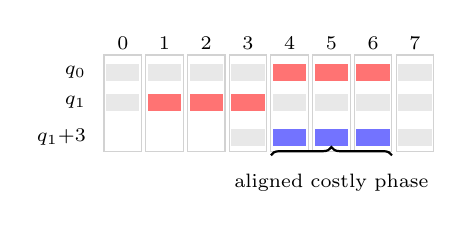
\begin{tikzpicture}[font=\scriptsize, x=5.3mm, y=5mm]
    \foreach \x in {0,...,7} {
      \node at (\x,1.75) {\x};
      \draw[gray!35] (\x-0.45,-1.0) rectangle (\x+0.45,1.45);
    }
    \node[anchor=east] at (-0.65,1) {$q_0$};
    \node[anchor=east] at (-0.65,0.25) {$q_1$};
    \foreach \x in {0,...,7} \fill[gray!18] (\x-0.4,0.78) rectangle (\x+0.4,1.22);
    \foreach \x in {0,...,7} \fill[gray!18] (\x-0.4,0.03) rectangle (\x+0.4,0.47);
    \foreach \x in {4,5,6} \fill[red!55] (\x-0.4,0.78) rectangle (\x+0.4,1.22);
    \foreach \x in {1,2,3} \fill[red!55] (\x-0.4,0.03) rectangle (\x+0.4,0.47);
    \node[anchor=east] at (-0.65,-0.65) {$q_1{+}3$};
    \foreach \x in {3,...,7} \fill[gray!18] (\x-0.4,-0.87) rectangle (\x+0.4,-0.43);
    \foreach \x in {4,5,6} \fill[blue!55] (\x-0.4,-0.87) rectangle (\x+0.4,-0.43);
    \draw[decorate, decoration={brace, amplitude=3pt}, thick]
      (3.55,-1.1) -- (6.45,-1.1) node[midway, below=3pt] {aligned costly phase};
  \end{tikzpicture}
  \caption{Why start offsets can increase sharing.  Red cells denote expensive traversal phases that do not overlap at zero offset; delaying $q_1$ by three global iterations aligns them (blue).  The offset changes time, not either query's logical levels.}
  \Description{Two query timelines have expensive phases at different global steps.  Delaying the second query shifts its expensive phase to coincide with the first.}
  \label{fig:phase-alignment}
\end{figure}


\subsection{Design Principles}

The observations lead to three principles that organize the rest of the paper.

\paragraph{P1: Share repeated neighborhood accesses exactly.}
The execution state must represent the active queries of each vertex, not only a query-oblivious union or cumulative visited set.  Exact membership lets the system read a shared neighborhood once without introducing unrelated query--edge work.

\paragraph{P2: Regularize the remaining query-state accesses.}
When broad frontiers make neighborhood sharing less selective, the engine should organize query values by graph vertex and aggregate them in a regular order.  This principle reduces effective access cost while preserving the same graph semantics.

\paragraph{P3: Schedule for realized sharing.}
Source similarity is useful only when it predicts simultaneous high-cost overlap.  The scheduler must consider relative traversal phases, batch queries with compatible overlap, and bound the delay introduced to create that overlap.

These principles explain why fusion alone is insufficient.  A global union without query membership violates P1; one fixed traversal strategy cannot satisfy both P1 and P2 across all frontier phases; and input-order batching ignores P3.  Sections~\ref{sec:overview}--\ref{sec:implementation} develop a system around these principles, while Section~\ref{sec:evaluation} assigns separate evidence to access-count reduction, access-cost reduction, and scheduling.
